\chapter{Utiliser Luke}

Luke est un logiciel permettant de visualiser un index créé avec Lucene. Après avoir téléchargé la version 6.3.0, nous avons exécuté le fichier \texttt{luke.sh} pour visualiser l’index créé avec la demo de Lucene visible sur la \autoref{img:luke}

\begin{figure}[H]
    \centering
    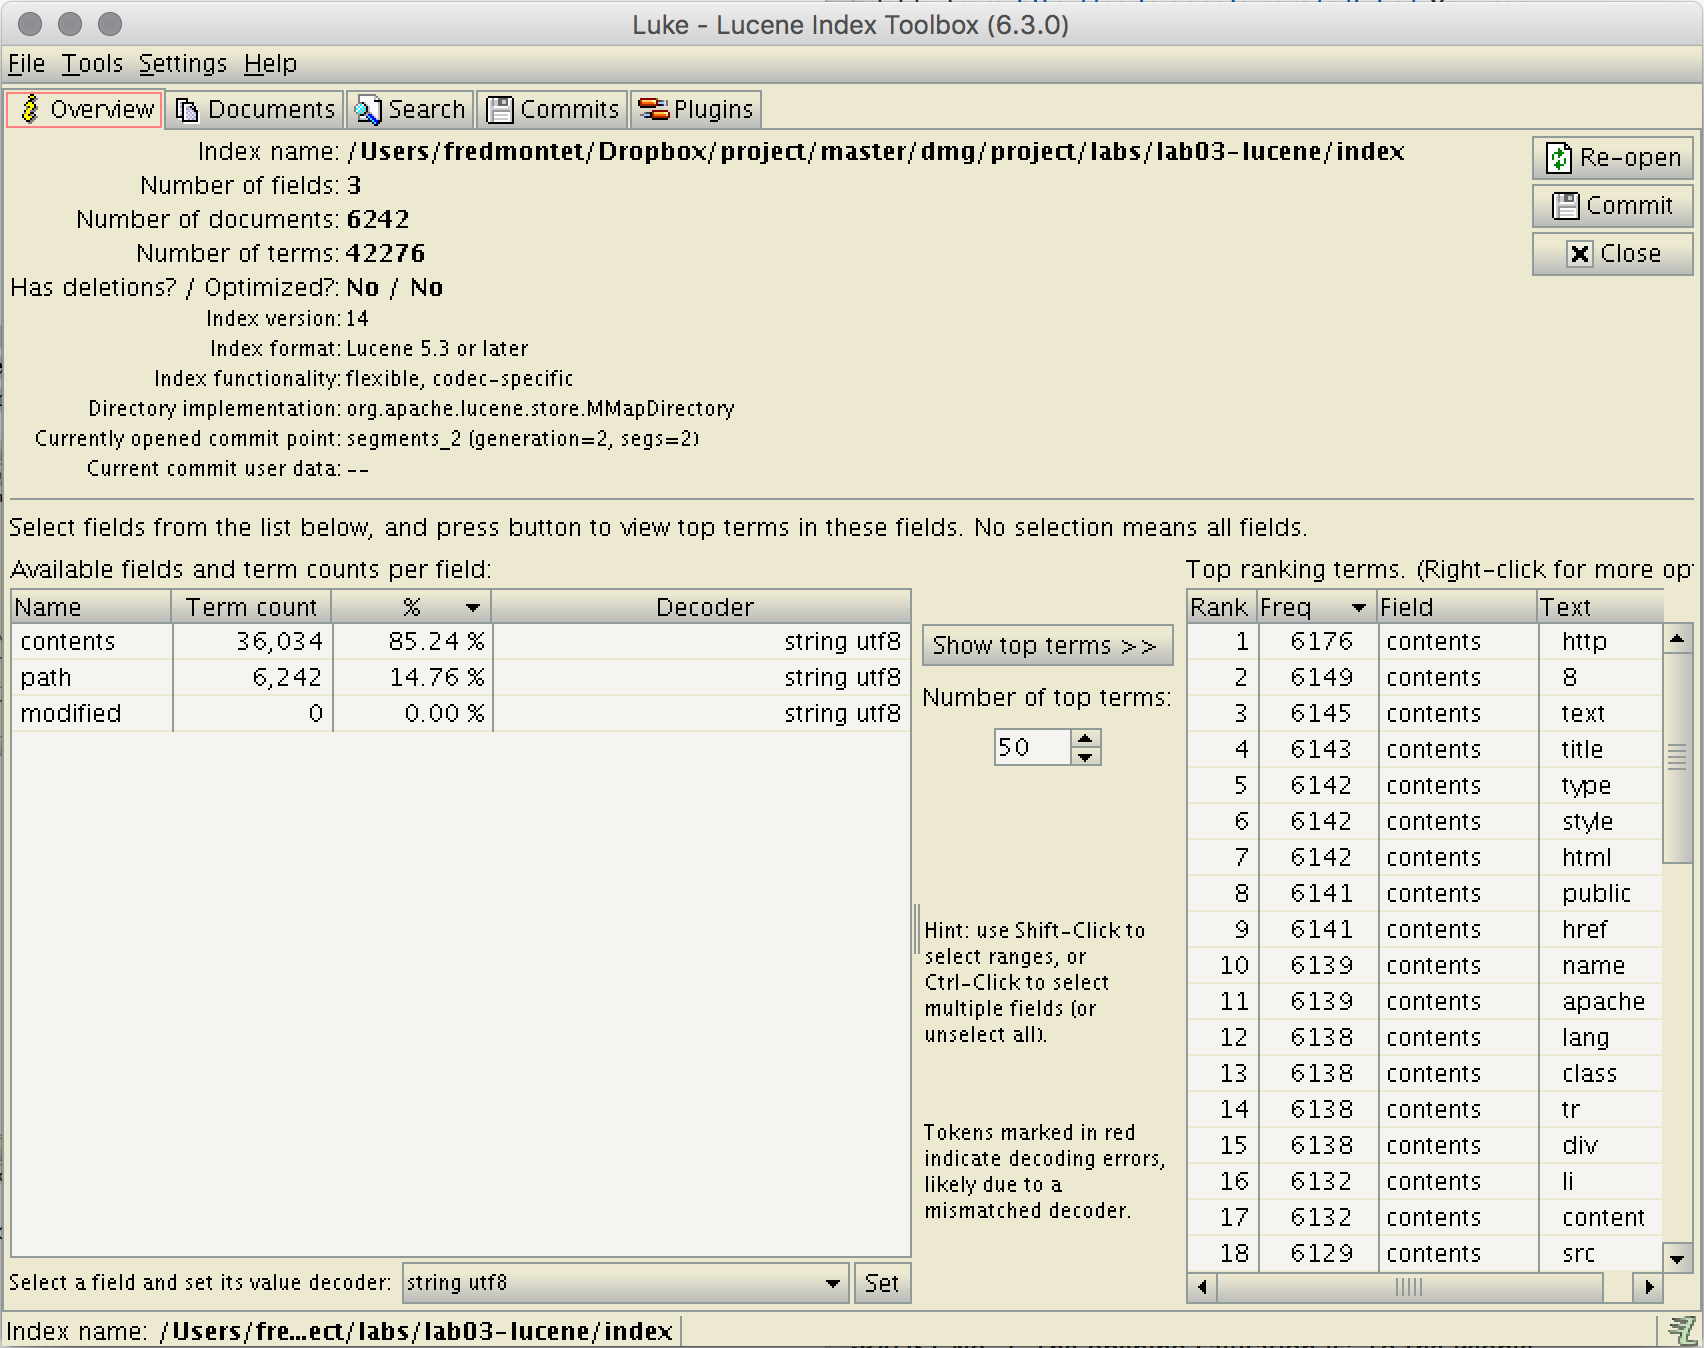
\includegraphics[width=0.7\linewidth, fbox]{img/luke.png}
    \caption{Interface de Luke avec l'index de la documentation de Lucene}
    \label{img:luke}
\end{figure}
